% ****** Start of file apssamp.tex ******
%
%   This file is part of the APS files in the REVTeX 4.2 distribution.
%   Version 4.2a of REVTeX, December 2014
%
%   Copyright (c) 2014 The American Physical Society.
%
%   See the REVTeX 4 README file for restrictions and more information.
%
% TeX'ing this file requires that you have AMS-LaTeX 2.0 installed
% as well as the rest of the prerequisites for REVTeX 4.2
%
% See the REVTeX 4 README file
% It also requires running BibTeX. The commands are as follows:
%
%  1)  latex apssamp.tex
%  2)  bibtex apssamp
%  3)  latex apssamp.tex
%  4)  latex apssamp.tex
%
\documentclass[%
reprint,
%superscriptaddress,
%groupedaddress,
%unsortedaddress,
%runinaddress,
%frontmatterverbose, 
%preprint,
%preprintnumbers,
%nofootinbib,
%nobibnotes,
%bibnotes,
amsmath,amssymb,
aps,
%pra,
%prb,
%rmp,
%prstab,
%prstper,
%floatfix,
]{revtex4-2}
\usepackage{adjustbox}
\usepackage{subfiles}
\usepackage{graphicx}% Include figure files
\usepackage{dcolumn}% Align table columns on decimal point
\usepackage{bm}% bold math
\usepackage{float}
\usepackage{mathtools}
\usepackage{xcolor}
\usepackage{physics}
\usepackage{dsfont}
\usepackage{tcolorbox}
\usepackage{float}
\usepackage{tensor}
\usepackage{subcaption}
\usepackage{hyperref}% add hypertext capabilities
%\usepackage[mathlines]{lineno}% Enable numbering of text and display math
%\linenumbers\relax % Commence numbering lines

%\usepackage[showframe,%Uncomment any one of the following lines to test 
%%scale=0.7, marginratio={1:1, 2:3}, ignoreall,% default settings
%%text={7in,10in},centering,
%%margin=1.5in,
%%total={6.5in,8.75in}, top=1.2in, left=0.9in, includefoot,
%%height=10in,a5paper,hmargin={3cm,0.8in},
%]{geometry}
\newcommand{\Hp}{\mathcal{H}}
\renewcommand{\thesection}{\arabic{section}}
\renewcommand{\thesubsection}{\thesection.\arabic{subsection}}
\renewcommand{\thesubsubsection}{\thesubsection.\arabic{subsubsection}}
\renewcommand{\figurename}{Fig.}
\renewcommand{\tablename}{Table}
\makeatletter
\renewcommand{\subsubsection}{%
	\@startsection
	{subsubsection}%
	{3}%
	{\z@}%
	{.8cm \@plus1ex \@minus .2ex}%
	{.5cm}%
	{\normalfont\small\centering}%
}
\makeatother
\renewcommand{\L}{\mathcal{L}}
\renewcommand{\O}{\mathcal{O}}
\newcommand{\f}[2]{\frac{#1}{#2}}
\newcommand{\p}{\partial}



\begin{document}
	
\title{Recurrent Neural Networks and Synthetic Gravitational Waves}
\author{Edvard B. Rørnes}
\email{e.b.rornes@fys.uio.no}
\author{Isak O. Rukan}
\email{icrukan@uio.no}
\affiliation{Institute of Physics, University of Oslo,\\0371 Oslo,  Norway}
\date{\today}

\begin{abstract}
	Gravitational waves, which are ripples in spacetime produced by cataclysmic astrophysical events such as black hole and neutron star mergers, present challenges for detection due to their faint signals often being buried by noise. The Laser Interferometer Gravitational-Wave Observatory (LIGO) has pioneered the detection of these waves, leveraging laser interferometry to measure tiny spacetime distortions. However, traditional detection methods face limitations in distinguishing weak GW signals from background noise.
	
	In this work, we explore the potential of neural networks (NNs) for GW detection, focusing on Recurrent Neural Networks (RNNs) to analyze untreated GW data obtained from publicly available datasets from \cite{gwosc}. Due to the low signal-to-noise ratio (SNR) of this data and the complexity of noise removal techniques, we instead generate synthetic GW data with controllable SNR for training and testing purposes. This approach allows us to evaluate the performance of our custom RNN implementation against the RNN framework provided by \texttt{tensorflow.keras}. While detection on untreated data remains challenging, the synthetic dataset allows for systematic evaluation and refinement of NN-based detection methods. Additionally, we provide a utility program\footnote{\href{https://github.com/EdvardRornes/FYS-STK4155/tree/main/Project3}{GitHub}} which automatically downloads and labels GW data when the signal duration is known, which may be useful for future work aimed at improving detection on real-world datasets.
\end{abstract}

\maketitle
%\tableofcontents

\section{Introduction}
Gravitational Waves (GWs) are the product of some of the most extreme events that occur in the universe. While in theory, just about any accelerating object produces GWs, they are so weak that they can only be detected from the most energetic and cataclysmic events \cite{ligo_gw_sources}. The only sources of detectable GWs with current technology are the mergers of black holes and neutron stars \cite{LIGOScientific:2007fwp}, where the immense masses and high velocities involved generate powerful ripples in spacetime. These ripples propagate outward and cause minute distortions in spacetime itself, which can be measured by highly sensitive instruments.

To date, the most advanced experiment to detect these waves is the Laser Interferometer Gravitational-Wave Observatory (LIGO). LIGO uses laser interferometry to measure the incredibly small displacements caused by passing gravitational waves. However, the signals from gravitational waves are often faint and easily overwhelmed by noise, making detection a difficult task.

Neural Networks (NNs) has become a powerful tool in this context. By training a NN on large datasets of both gravitational wave signals and background noise, these models can learn to distinguish between genuine gravitational wave signals and random noise. This, in theory, may allow for more accurate detection and classification of GW events, even in the presence of significant interference, and may be the future of GW detection \cite{Marx:2024wjt, skliris2024}. NNs can be trained to recognize patterns in the data that correspond to the characteristic signatures of GWs, improving both the efficiency and reliability of detection algorithms. With the growing amount of data from observatories like LIGO, NNs are playing an increasingly important role in identifying new events and advancing our understanding of the universe.

In this work we attempt to detect GWs on untreated data from \cite{gwosc} by building our own Recurrent Neural Network (RNN), along with using \texttt{tensorflow.keras}' RNN to test against our own. To do this we created a program which automatically labels GW files granted that the user knows the duration of the GW signal. The performance on the untreated data from \cite{gwosc} is quite poor due to the untreated data having a signal to noise ratio (SNR) which is far too low for our programs. The process of removing noise from GW is quite advanced, and requires state of the art techniques. Due to time constraints and lack of expertise in this field, we instead created a simple program which generates synthetic GW data. This allowed us to control the SNR and focus on training neural networks on processed data, which simplifies the task vastly and allows us to evaluate our RNN's performance. This however still led to poor performance for both the RNN's, only yielding acceptable results is near trivial tasks where the SNR $\sim100$. After attempting many different parameter combinations, we eventually ended up using keras' Convolutional Neural Network (CNN) instead.

This document begins by introducing some of the necessary theory and techniques required to understand the results in section \ref{sec:theory}. We then go on to discuss our implementation of the various NN's along with some of the other tools we have used in section \ref{sec:implementation} along with a short discussion of the challenges of GW detection in section \ref{sec:challenges}. Finally, ending on the results obtained.

\section{Theory}
\label{sec:theory}
\subsection{Gravitational Waves}
We will simply give a quick introduction to GWs. For a more detailed analysis, please see any graduate level textbook on general relativity, e.g.~\cite{Carroll} or \cite{Wald}.

As mentioned, GWs are ripples in spacetime caused by the acceleration of massive objects, such as merging black holes or neutron stars. For sufficiently small ripples, or for an observer sufficiently far away from e.g.~a black hole merger, the GWs are accurately described by first order perturbations of a flat spacetime described by the Minkowski metric, $\eta_{\mu\nu}$, with a small perturbation:
\begin{align}
	g_{\mu\nu}=\eta_{\mu\nu}+h_{\mu\nu},\quad|h_{\mu\nu}|\ll1,
\end{align}
where the metric signature is $(-,+,+,+)$. The Einstein field equations (EFE) are given by
\begin{align}
	G_{\mu\nu}=8\pi GT_{\mu\nu},
	\label{eq:EFE}
\end{align}
where $G_{\mu\nu}$ is the Einstein tensor which depends solely on the metric $g_{\mu\nu}$, and $T_{\mu\nu}$ is the stress-energy tensor. Applying the perturbed metric to \eqref{eq:EFE} one can show that to first order this gives the linearized EFE \cite{Carroll}:
\begin{align}
	-16\pi T_{\mu\nu}&=\Box h_{\mu\nu}-\p_\mu\p^\rho h_{\nu\rho}-\p_\nu\p^\rho h_{\mu\rho}\nonumber\\
	&+\eta_{\mu\nu}\p^\rho\p^\sigma h_{\rho\sigma}+\p_\mu \p_\nu h-\eta_{\mu\nu}\Box h,
	\label{eq:LEFE}
\end{align}
where $h\equiv \tensor{h}{^\mu_\mu}=\eta^{\mu\nu}h_{\mu\nu}$ is the first order trace of $h$ and $\Box$ is the flat space d'Alembertian. Note that we do not perturb $T_{\mu\nu}$ since it is in fact a perturbation itself. Now this equation here is quite complicated, however due to a symmetry in the original Lagrangian one has a so-called \textit{gauge freedom}, i.e.~a set of transformations which leave the Lagrangian invariant. This can be used to vastly simplify the equations heavily. A common choice is the Lorenz gauge: $\p^\mu h_{\mu\nu}=0$. Using this we can reduce \eqref{eq:LEFE} to the much simpler differential equation
\begin{align}
	\Box h_{\mu\nu}=-16\pi T_{\mu\nu}.
\end{align}
Specializing to the case corresponding to a vacuum ($T_{\mu\nu}=0$) then we simply have a plane wave equation
\begin{align}
	\Box h_{\mu\nu}=0,\implies h_{\mu\nu}=C_{\mu\nu}e^{ikx},\quad k_\mu k^\mu=0,
\end{align}
where
\begin{align}
	C_{\mu\nu}=\begin{bmatrix}
		0&0&0&0\\
		0&h_+&h_\times&0\\
		0&h_\times&-h_+&0\\
		0&0&0&0
	\end{bmatrix},
\end{align}
for a GW traveling along the $z$-axis. The details for how this is derived and why it must take on this form is spelled out in \cite{Carroll}. $h_+$ and $h_\times$ correspond to the ``plus'' and ``cross'' polarization respectively, which determine how the gravitational waves stretch and compress the spacetime it passes through. 

The stretching and compression from these polarizations are what is measured by observatories such as LIGO and Virgo. These displacements are often given as the dimensionless quantity \textbf{strain}, which is simply given by $\Delta L/L$ where $L$ is the effective length of the detector, and $\Delta L$ is the measured change in $L$ as the GW passes by. Note that in the case of detection, $L$ is not simply the length of the detectors themselves, as they use mirrors to cause the beams of light to bounce back and forth multiple times, effectively increasing the length of the detector.


\subsection{Recurrent Neural Networks}
\label{sec:RNNs}
The Recurrent Neural Networks (RNNs) are a class of neural networks specifically designed to handle sequential data or data with temporal dependencies. Unlike traditional Feed Forward Neural Networks, RNNs are capable of ``remembering'' information from previous time steps. This is done through the so called `hidden state', which acts as a form of memory by retaining information about prior computations. The hidden state is essentially an array of data that is updated at each time step based on the input data and the previous hidden state. Although this enables RNN to access the temporal dependencies of the data at hand, it greatly increases the computation time compared to that of the FFNN. The standard RNN consists of only one hidden layer, but it is certainly possible to have more than one hidden layer. In fact, this is commonly referred to as the stacked RNN (SRNN), and we will arrive at this neural network further down. However, firstly, we present the structure and general algorithm for the RNN.

\subsubsection{Structure}
The RNN processes input sequentially, with information flowing step-by-step from the input to the output. This is done with the introduction of a hidden state \(h_{t}\), where the subscript denotes at time \(t\). The network can be summarized by the following two equations \cite{tallec2017unbiasingtruncatedbackpropagationtime}:
\begin{subequations}
\begin{align}
	h_{t} &= \sigma^{(h)}\left(W_{hx}X_{t} + W_{hh}h_{t-1}  + b_{h}\right), \label{eq:hidden_state_RNN} \\
	\tilde{y}_{t} &= \sigma^{(\text{out})}\left(W_{yh}h_{t} + b_{y}\right).	\label{eq:output_RNN}
\end{align}
\end{subequations}
Here, \(\sigma_h\) and \(\sigma_{\text{out}}\) is the activation function for the hidden layer and the output layer respectively. \(W_{xh}\) is the weight from input to hidden layer, \(W_{hh}\) the hidden layer, \(W_{yh}\) the output layer and \(\tilde{y}\) the output of the RNN. Let now \(t\) be divided into a discrete set of times \((t_i)_{i\in N}\). Substituting \eqref{eq:hidden_state_RNN} into itself recursively leads to a formula for computing \(h_{t_n}\):
\begin{align}	\label{eq:hidden_state_computation_RNN}
	h_{t_n} = \sigma^{(h)}\biggl( W_{hx}X_{t_n} &+ W_{hh}\sigma_h \biggl( W_{hx}X_{t_{n-1}} \notag\\
	&+ W_{hh}\sigma_h \left(\dots + b_h\right) + b_h\biggr) 
	+b_h\biggr)
\end{align}
This shows that the hidden state at time \(t_n\) is dependent on the input \(X_{t}\) for \(t\in[0, t_n]\), i.e.~all previous times. 

\subsubsection{General Algorithm}
Consider some general data output \(y\), of shape \((N, p_{\text{out}})\) and some data input \(X\), of shape \((N, p_{\text{in}})\), where \(N\) corresponds to the total amount of time points, and \(p_{\text{out}}, \ p_{\text{in}}\) the dimension of the output and input, respectively. Generally, \(X\) could correspond to a large sampling frequency in time, making the computation of the hidden state \(h_t\) in \eqref{eq:hidden_state_computation_RNN} computationally demanding. One typical way of dealing with this is to split the data into `windows' of size \(N_{W}\) in time. These windows should generally overlap, such that no temporal dependencies across windows are left out. 

Splitting the data into windows, we define the hidden state for window \(n\) as:
\begin{align}
	h_{n} &= \sigma^{(h)}\left( W_{hx}X_{n} + W_{hh}h_{n-1} + b_{h} \right) \notag \\
	&\equiv \sigma^{(h)}(z_{n})
\end{align}
where \(X_{n}\) is the \(n\)-th window.

\subsubsection{Backpropagation Through Time}
The error between \(y\) and the predicted output \(\tilde{y}\), is given by some chosen loss function \(L(y, \tilde{y})\),
\begin{align}	
	L(y,\tilde{y}) = \frac{1}{N}\sum\limits_{n=1}^{N} l(y_{n}, \tilde{y}_n),
\end{align}
where \(l\) is some error-metric. 
For some learning rate \(\eta\), the standard update rule for the weights and biases is given by:
\begin{align}
	W\leftarrow W-\eta \frac{\partial L}{\partial W},\quad b\leftarrow b-\eta \frac{\partial L}{\partial b}.
\end{align}
This transformation may be extended using optimization methods aimed at handling exploding gradient, faster convergence, avoiding local minimas, etc. We covered three of these optimization methods in \cite{project2}; the root mean squared propagation (RMSprop), the adaptive gradient (AdaGrad) and the adaptive moment estimation (Adam). 

Compared to FFNN, computing the gradient of \(L\) with respect to the weights leads to a somewhat more complicated expression due to the temporal dependencies between the hiden states. This can be seen by writing out the partial derivative of the loss function with respect to the weight \(W\),  being either \(W_{hx}\) or \(W_{hh}\) (cf. \cite{superGood}):
\begin{align}
	\frac{\partial L}{\partial W} &= \sum_{n=1}^{N}\frac{\partial L}{\partial \tilde{y}_{n}} \frac{\partial \tilde{y}_{n}}{\partial W}\\
	&= \sum_{n=1}^{N}\frac{\partial L}{\partial \tilde{y}_{n}} \frac{\partial \tilde{y}_{n}}{\partial h_{n}}\frac{\partial h_{n}}{\partial W},
\end{align}
where we can use backpropagation through time (BPTT) to write \cite{superGood}:
\begin{align}	\label{eq:dL_dW_bare}
	\frac{\partial L}{\partial W} &= \sum_{n=1}^{N}\sum_{k=1}^{n}\frac{\partial L}{\partial \tilde{y}_{n}} \frac{\partial \tilde{y}_{n}}{\partial h_{n}} \frac{\partial h_{n}}{\partial h_{k}} \frac{\partial h_{k}}{\partial W}.
\end{align}
Applying the chain rule in succession we obtain: 
\begin{align}
	\frac{\partial h_n}{\partial h_k} &= \frac{\partial h_n}{\partial h_{n-1}} \frac{\partial h_{n-1}}{\partial h_{n-1}} ... \frac{\partial h_{k+1}}{\partial h_{k}} \notag \\
	&= \left[ W_{hh}^{T}\cdot\sigma'_{h}(z_n) \right]\left[ W_{hh}^{T}\cdot\sigma'_{h}(z_{n-1}) \right] ... \left[ W_{hh}^{T}\cdot\sigma'_{h}(z_{k+1}) \right] \notag\\
	&= \prod_{j=k+1}^{n}\left[ W_{hh}^{T}\cdot\sigma'_{h}(z_{j})\right],
\end{align}
meaning that
\begin{align}	\label{eq:dL_dW_alone}
	\frac{\partial L}{\partial W} &= \sum_{n=1}^{N}\sum_{k=1}^{n}\frac{\partial L}{\partial \tilde{y}_{n}} \frac{\partial \tilde{y}_{n}}{\partial h_{n}} \prod_{j=k+1}^{n}\left[ W_{hh}^{T}\cdot\sigma'_{h}(z_{j})\right] \frac{\partial h_{k}}{\partial W}.
\end{align}

Up until now we have considered only one hidden layer. Implementing the stacked RNN is done by essentially creating a hidden state for each `stack' of RNN. The output of the stacked RNN is computed by feeding the hidden states to each other in succession, starting from the first hidden layer. The \(l\)-th hidden states in some time window \(n\) are given by
\begin{align}
	h^{l}_{n} = \begin{cases}
		\sigma^{(h)}\left( W_{hx}^{1}X_{n} + W_{hh}^{1}h_{n-1}^{1} + b_{h}^{1}\right), &l=1, \\
		\sigma^{(h)}\left( W_{hx}^{l}h_{n}^{l-1} + W_{hh}^{l}h_{n-1}^{l} + b_{h}^{l}\right), &l\geq 2,
	\end{cases}
\end{align}	
and the output of the stacked RNN in time window \(n\) as
\begin{align}
	\tilde{y}_{n} &= \sigma^{(\text{out})}\left( W_{yh}h^{L}_{n} + b_{y} \right),
\end{align}
with \(L\) being the total amount of hidden layers. 
Here, the dimensions are \(W^{l}_{hx}\in\mathbb{R}^{d_{l}\times d_{l-1}}\), \(W^{l}_{hh}\in\mathbb{R}^{d_{l}\times d_{l}}\), with \(d_l\) being the dimension of the \(l\)-th hidden state, \(l_0\) the dimension of the input and \(l^{L}\) the dimension of the output. The BTT algorithm for a stacked RNN takes on the same form, except that we now have \(L\) hidden states. 


To update the weights, we define the errors:
\begin{align}
	\delta^{k,l}_{hh}\equiv \frac{\partial h_{k}^{l}}{\partial W_{hh}^{l}}, \ \delta^{k,l}_{hx}\equiv \frac{\partial h_{k}^{l}}{\partial W_{hx}^{l}}.
\end{align}
These errors can be computed recursively through time. For \(\delta^{k,l}_{hh}\), 
\begin{align}
	\delta^{1,l}_{hh} &= 0, \notag\\
	\delta^{2,l}_{hh} &= \sigma'_{h}(z_2^{l}) h_1^{l},  \notag\\
	\delta^{3,l}_{hh} &= \sigma'_{h}(z_3^{l}) \left( h_2^{l} + W_{hh}\sigma'_{h}(z_2^{l})h_1^{l} \right), \\
	&\dots, \notag \\
	\delta^{k,l}_{hh} &= \sigma'_{h}(z_{k}^{l}) \left( h_{k-1}^{l} + W_{hh}\delta^{k-1,l}_{hh}\right).
\end{align}
and for \(\delta^{k,l}_{hx}\),:
\begin{align}
	\delta^{k,1}_{hx} &= \sigma'(z_{k}^{1})X_{k}, \notag\\
	\delta^{k,2}_{hx} &= \sigma'_{h}(z_{k}^{2}) \left( h_{k}^{1} + W^{2}_{hh}\sigma'(z_{k-1}^{2})X_{k} \right),  \notag\\
	% \delta^{k,3}_{hx} &= \sigma'_{h}(z_{k}^{3}) \left( h_{k}^{2} + W_{hh}^{3}\delta^{k,2}_{hx} \right), \\
	&\dots, \notag \\
	\delta^{k,l}_{hx} &= \sigma'_{h}(z_{k}^{l}) \left( h_{k}^{l-1} + W_{hh}^{l}\delta^{k-1,l}_{hx}\right).
\end{align}

We can then summarize how the hidden-layer weights and biases are updated (cf. \cite{superGood}):
\begin{subequations}	\label{eq:gradients_hidden}
	\begin{align}
		\frac{\partial L}{\partial W_{hh}^{l}} &= \sum_{n=1}^{N}\sum_{k=1}^{n}\frac{\partial L}{\partial h_{n}^{l}}  \left[ \prod_{j=k+1}^{n} \sigma'_{h}(z_{j}^{l})W_{hh}^{l}\right] \delta^{k,l}_{hh}, \\
		\frac{\partial L}{\partial W_{hx}^{l}} &= \sum_{n=1}^{N}\sum_{k=1}^{n}\frac{\partial L}{\partial h_{n}^{l}}  \left[ \prod_{j=k+1}^{n} \sigma'_{h}(z_{j}^{l})W_{hh}^{l}\right] \delta^{k,l}_{hx}, \\
		\frac{\partial L}{\partial b_{h}^{l}} &= \sum_{n=1}^{N}\sum_{k=1}^{n}\frac{\partial L}{\partial h_{n}^{l}}  \left[ \prod_{j=k+1}^{n} \sigma'_{h}(z_{j}^{l})W_{hh}^{l}\right] \sigma'_{h}(z_k^l),
	\end{align}
\end{subequations}
since \(\partial h^{l}_{n}/\partial b_{h}^{l} = \sigma'_{h}(z_k^l)\). For the output layer, \(\partial h_n/\partial W_{yh}\) is only non zero of \(n=N\), hence
\begin{subequations}	\label{eq:gradients_out}
	\begin{align}
		\frac{\partial L}{\partial W_{yh}} &= \frac{\partial L}{\partial \tilde{y}_{n}} \frac{\partial z_N}{\partial h_{n}} \sigma'_{\text{out}} h_{N}, \\
		\frac{\partial L}{\partial b_{y}} &= \frac{\partial L}{\partial \tilde{y}_{n}} \frac{\partial z_N}{\partial h_{n}} \sigma'_{\text{out}}.
	\end{align}
\end{subequations}

The dependency for each error term \(\delta^{k,l}\) on `past' error terms leads to a much greater computation time, compared to that of FFNN. Every gradient computation needs an additional propagation through all time-windows. This can lead to gradients blowing up due to only (relatively) minor errors. However, there are multiple ways of resolving this issue. Perhaps the most obvious one is to simply truncate the amount of terms in the algorithm, commonly referred to as `truncated backpropagation through time' (see e.g.~\cite{tallec2017unbiasingtruncatedbackpropagationtime}). Apart from that it is an actual simplification, it has the immediate consequence of ignoring long-term dependencies of the data, which in some cases is just the type of information you do not want your model to train on.

\subsection{Convolutional Neural Networks}
Convolutional neural networks (CNNs) are specialized deep learning architectures that process data with a spatial structure, such as images or signals. The core operation of CNNs is the convolution, defined for a 1D input signal $f[i]$ and a filter kernel $g[n]$ as:
\[(f*g)[i]=\sum_{n}f[n]g[i-n].\]
For a 2D input, the convolution is given by:
\[(f*g)[i,j]=\sum_{m}\sum_{n}f[i-m,j-n]g[m,n],\]
where $f[i,j]$ is the input pixel value, and $g[m,n]$ is the filter kernel.

The convolution operation captures local patterns, such as edges or textures, which are passed through an activation function. The next layers of the CNN extract increasingly abstract features.

To reduce dimensionality and improve computational efficiency, CNNs often include pooling layers, such as max-pooling:
\[\text{MaxPooling}(x)=\max(x_{\text{window}}),\]
where $x_{\text{window}}$ refers to a subset of the input.

The high-level features extracted by convolutional and pooling layers are processed by fully connected layers to make predictions, such as classifying an image or detecting a signal. In the case of GWs, these convolutional layers essentially work to filter out most the background noise, leaving the signal mostly intact. 



\subsection{Additional Techniques}
\subsubsection{Regularization \& Loss Function}
We used $L^2$ regularization for all our results. We refer to \cite{project1} for an introduction. The loss function considered for all our results was the weighted binary-cross entropy with this additional $L^2$ regularization:
\begin{align}
	L&=-\frac1N\sum_{i=1}^N\left[S_\text{CW}\,y_i\ln(\hat{y}_i)+(1-y_i)\ln(1-\hat{y}_i)\right]\nonumber\\
	&+\lambda\sum_{i=1}^Nw_i^2
\end{align}
where $S_{\text{CM}}$ is the signal class weight and the noise class weight has been normalized to unity.

\subsubsection{Gradient Clipping}
A common method for dealing with exploding gradients, is the method of gradient clipping (see e.g.~\cite{Goodfellow-et-al-2016}). This method prevents checks whether the magnitude of the gradient is moving past a certain threshold. If this is true it truncates the current gradient. This can be summarized as:
\begin{align}	\label{eq:clipping}
	\nabla L \rightarrow \frac{\epsilon}{||\nabla L||}\nabla L\quad\text{if}\quad||\nabla L|| > \epsilon.
\end{align}

\subsubsection{Early Stopping}
We opted into using early stopping for the majority of our parameter scans. Given that our program did not improve in a certain number of epochs (between $15\%$ and $40\%$ depending inversely on the number of epochs), and the loss was sufficiently high, we ended the learning process early. If the loss was sufficiently good, we however still kept on going, in the hopes that we would be able to improve the model further. This is mostly done to not waste time on parameter combinations which perform poorly. 

\subsubsection{Dynamic Class Weights}
To handle the large class imbalance between the noise and gravitational events, we introduced a dynamic class weight adjustment based on a hyperparameter $\phi$. Given the label array $\textbf{l}$, if we define $l_i=1$ when there is a signal, and $l_i=0$ when there is only noise and normalize the noise class weight to $1$, then a simple way to compute a linear dynamical weights for the signal class is:
\begin{align}
	S_{\rm CW}&=\left[\phi-(\phi-1)\frac{\varE}{E}\right]\times\left[\frac{{\rm len}(\textbf{l})}{\sum_i l_i}-1\right]
\end{align}
where $S_{\rm CW}$ refers to the signal class weight (GWs in our case), $\varE$ is the current epoch and $E$ is the total number of epochs. The right bracket is just the factor which would give you balanced class weights, i.e. the program is equally punished for only predicting either of the classes. The factor in the left bracket is then just a linearly decreasing factor going from $\phi$ to $1$ as $\varE\to E$. This essentially gives an early boost to the signal class, and gradually converges to a balanced class weight system where the NN would perform equally poorly from predicting all in either of the classes. A simple example is shown in Fig. \ref{fig:DynamicCW}. Note that the noise-signal label ratio is \textit{not} SNR, one refers to the time axis in the case of GW (i.e.~the percentage of time there is a signal), whilst the latter refers to the strain-to-noise ratio (i.e.~roughly how visible the signal is at any given time). Dynamical class labels are important in our case since GW events are so rare. Due to this the program may simply decide that it is best not to predict the signal class at all, as it is much more likely to be punished for ever attempting to `guess' GWs. Thus dynamical weights are a way to reduce the effects of this particular problem.
\begin{figure}[ht!]
	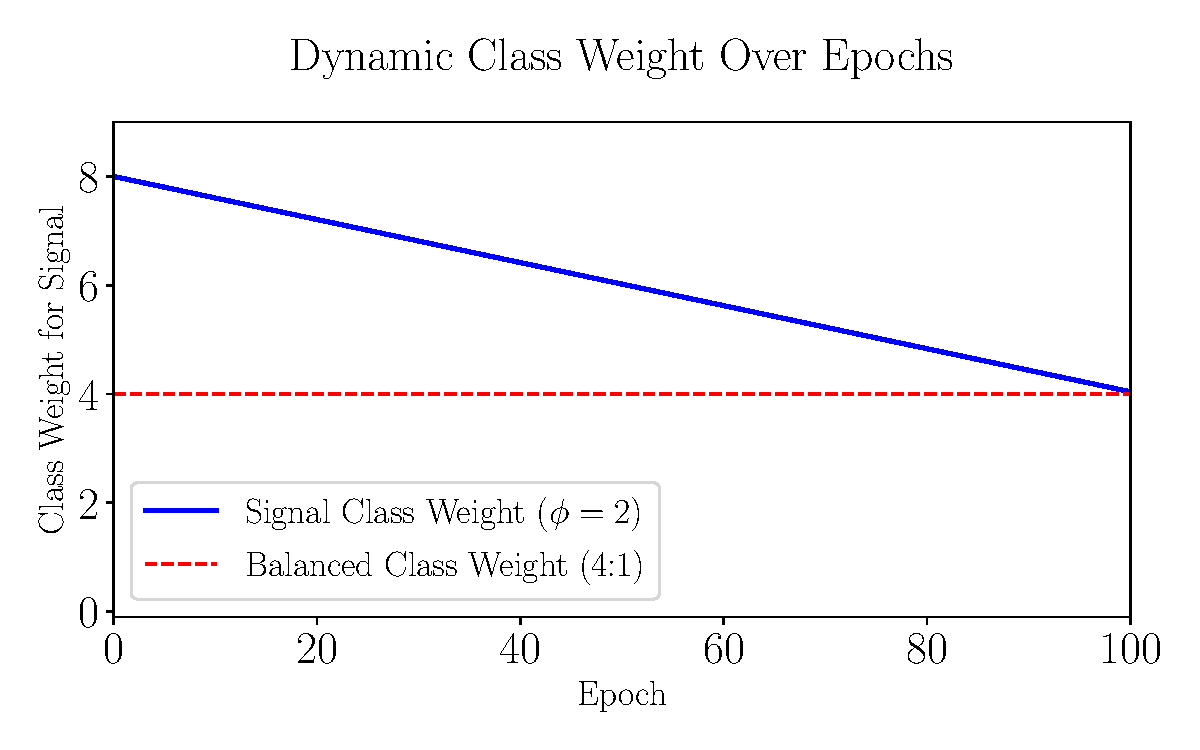
\includegraphics[width=0.49\textwidth]{Figures/DynamicCW.pdf}
	\caption{Dynamic class weight shown for a simple example with $\phi=2$ where we have a 4:1 noise-signal label ratio over 100 epochs.}
	\label{fig:DynamicCW}
\end{figure}

\subsubsection{Wavelet Transforms}
Wavelet transforms are mathematical tools used to analyze signals by decomposing them into time-frequency components. A wavelet transform applies scaled and shifted versions of a so-called \textit{mother wavelet} function, $\psi(t)$, to a signal. The continuous wavelet transform (CWT) of a signal $f(t)$ is defined as:
\[W(a,b)=\int_{-\infty}^{\infty}f(t)\psi_{a,b}(t)\,dt,\]
where $\psi_{a,b}(t)$ is the scaled and shifted wavelet:
\[\psi_{a,b}(t)=\frac{1}{\sqrt{|a|}}\psi\left(\frac{t-b}{a}\right),\]
with $a>0$ representing the frequency and $b$ the time shift.  

In the discrete wavelet transform (DWT), the scale and translation are discretized, typically as $a=2^j$ and $b=k\cdot2^j$, where $j$ and $k$ are integers. The DWT is computed as:
\[W[j,k]=\sum_{n}f[n]\psi_{j,k}[n],\]
making it computationally efficient for practical applications like feature extraction or de-noising. 

Unlike traditional Fourier transforms, which decompose a signal into sine and cosine waves of different frequencies, wavelets allow for both time and frequency localization. This makes them particularly useful for analyzing non-stationary signals, such as gravitational waves or audio signals, where the frequency content changes over time. In the context of neural networks, wavelet transforms are often used as a pre-processing step to reduce noise, extract meaningful features, or compress data, thereby potentially improving the performance.

\section{Implementation}
\label{sec:implementation}
We implemented a program which downloads the data from \cite{gwosc}, and when given the duration of the GW signal of interest, automatically labels the data accordingly. Our definition for `duration' of an event is rather arbitrary. What we did is simply look at a relevant research paper (found for each event at \cite{gwosc_all_events}) which contains plots of the treated data and made an educated guess for where it would be reasonable to detect it. Further we made a class \texttt{GWSignalGenerator}, which adds a synthetic GW signal to any arbitrary sequence, and adds corresponding labels to the dataset. This class has a lot of options, such as spin factors and amplitude factors for how much the signal should spike up, generating random events, etc. and was meant to simulate what GW event strain data looks like. Originally this program was meant to be our test runs before working with the real deal. However due to the complicated nature of detecting GWs, this ended up being what the NNs worked with instead. We explain the reasoning for this in the next section.

\subsection{The Neural Networks}
We have implemented two classes, \texttt{RNN} and \texttt{KerasRNN}, both of which inherits from a parent class called \texttt{NeuralNetwork} which contains methods handling saving data (\texttt{save\_data}), 
scaling and splitting data (\texttt{store\_train\_test\_from\_data}), and dividing the data into sequences (\texttt{prepare\_sequences\_RNN}). The class \texttt{RNN} is our own implementation of the stacked RNN architecture described in section \ref{sec:RNNs}, using the equations in \eqref{eq:gradients_hidden} and \eqref{eq:gradients_out} when training. On the other hand, the class \texttt{KerasRNN}, uses \texttt{keras}'s RNN \cite{keras_recurrent_layers}. Common to both classes are their public methods—\texttt{train}, \texttt{predict}, \texttt{cross\_validate} and \texttt{calculate\_loss}—which function as their names suggest. Both classes are initialized with key parameters, including a hidden-layer activation function, an output-layer activation function, a scaler type, and an optimizer, which can be set to plain gradient descent, Adagrad, RMSprop, or Adam. During training, the models require the input data, the number of epochs, batch size, window size, and optionally a clip value for gradient clipping, as implemented in \eqref{eq:clipping}. For details on the specific file structure, we refer to the README file at \href{https://github.com/EdvardRornes/FYS-STK4155/tree/main/Project3}{project 3}.

A program which uses \texttt{tensorflow.keras}' SimpleRNN was then implemented and parameter scans with the following parameters were performed:
\begin{itemize}
	\item $N\in\{10,25,50,100\}$
	\item $\phi\in\{1.0,1.1,...,1.5\}$
	\item $\lambda\in\{10^{-10},10^{-9},...,10^{-1}\}$
	\item $\eta\in\{10^{-4},5\times10^{-4},...,10^{-1},5\times10^{-1}\}$
\end{itemize}
where $N$ is the number of epochs. Due to the program being incredibly slow, we only ended up using the Adam optimizer, and only managed to finish half the parameter scan with $N=100$. Similarly, due to spending much time implementing our custom RNN, we only had time to perform a few parameter combinations. The performance of these were however so poor -- even with an extremely high SNR on the synthetic signal -- that they are not worth mentioning. This is likely due to mistakes in the implementation which we did not manage to fix.

The implementation keras RNN consist of starting with 5 separate signals which we generate, and perform $5$-fold cross validation on them. Within each training loop we again split the training data into a validation set. Since keras does not support dynamical class weights, we needed to perform the fitting with a single epoch, but still loop over each of these fittings $N$ number of times. We then perform the training and validate after each epoch. Every time we reach a new best validation loss, we save the weights and continue with them the next epoch. The model is then tested with the remaining test set with the best weights and the data corresponding to the run is saved to a \texttt{.pkl} file to be used later. Due to the program running very slowly, we saved a separate file for each parameter combination, and later used another program to merge all this data into larger data files.

Due to a massive lack of performance to the RNN's, we decided to include an implementation of keras' CNN's as well. This was done by... We then ran a small parameter scan due to time constraints where we included the following parameters: ... As before, we did not do this with the actual GW data, and instead opted into using our own signal generator class.

\section{Challenges}
\label{sec:challenges}
As we have mentioned prior, we did not end up using either of the RNN's nor the CNN on actual GW data, or at least not long enough to gather any meaningful results. The reason for this is simple; gravitational wave detection is very difficult! All the NN's simply ended up just randomly guessing due to the near impossibility of the task, so we just want to showcase how difficult this actually is.

Consider for example Fig.~\ref{fig:GW170104} which shows the raw strain data measured by the H1 LIGO detector surrounding the event GW170104 acquired from \cite{gwosc}. The small partition in red is where the GW signal was detected by both LIGO detectors and Virgo, whilst the rest is simply noise. This event has a roughly average peak SNR $\sim13$ (after treatment) and a rather common duration of roughly $0.04\,$s, so this would be around what would be expected of a NN to be able to detect. Whilst the strain here is of the order $10^{-18}$, after cleaning the data, \cite{LIGOScientific:2017bnn} shows that the actual strain stemming from the GW event peaks around $10^{-21}$. Thus the unfiltered SNR of the raw data is $\lesssim10^{-3}$. Clearly it is unreasonable to give this to a NN and expect it to learn anything, and this is even with data which is over a relatively short timespan of under 20 seconds. Note that even if we picked the GW with highest (treated) SNR, this is only $\sim3$ times higher than this particular example. Thus even in this most ideal case, we still have a raw data SNR which is at best $\sim10^{-2}$.

\begin{figure}[ht!]
	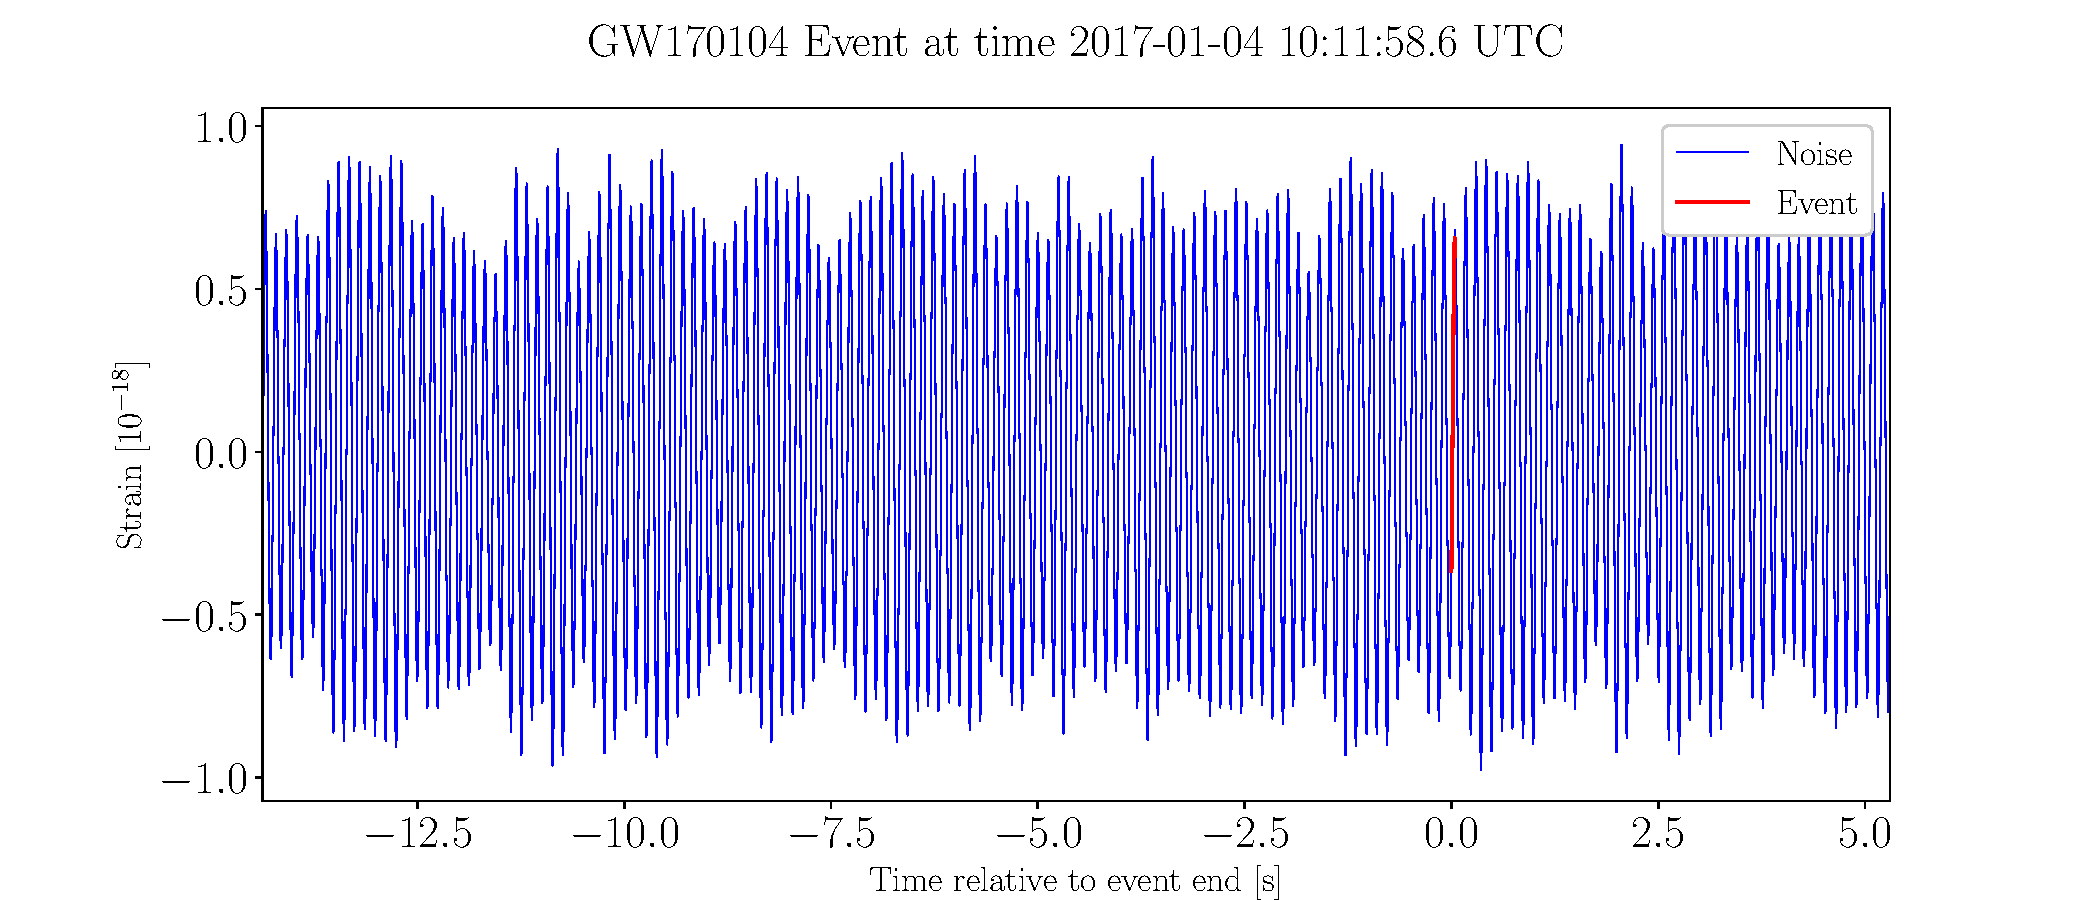
\includegraphics[width=0.5\textwidth]{Figures/GW170104GWEvent.pdf}
	\caption{Raw strain data for GW170104 v2 from the H1 LIGO detector \cite{gwosc}. Blue corresponds to noise whilst red is where the GW event has been detected.}
	\label{fig:GW170104}
\end{figure}

What academics do is they remove all the noise from known sources which occur at this time, e.g. seismic activity, local disturbances and afterwards perform a Bayesian analysis of the data to determine the properties of the source \cite{LIGOScientific:2017bnn}. Finally, they reconstruct the signal using the found properties and check against the original data. For this particular event, they arrived at the signal shown in Fig. \ref{fig:GW170104Reconstructed} which has a background noise $\sim10^{4}$ times smaller. This is clearly much easier to work with than the raw data, and a much more realistic task for a NN to be able to detect. However at this point all the work has already been done, and requires far more work than we can manage given our lack of expertise and time for this project.

\begin{figure}[ht!]
	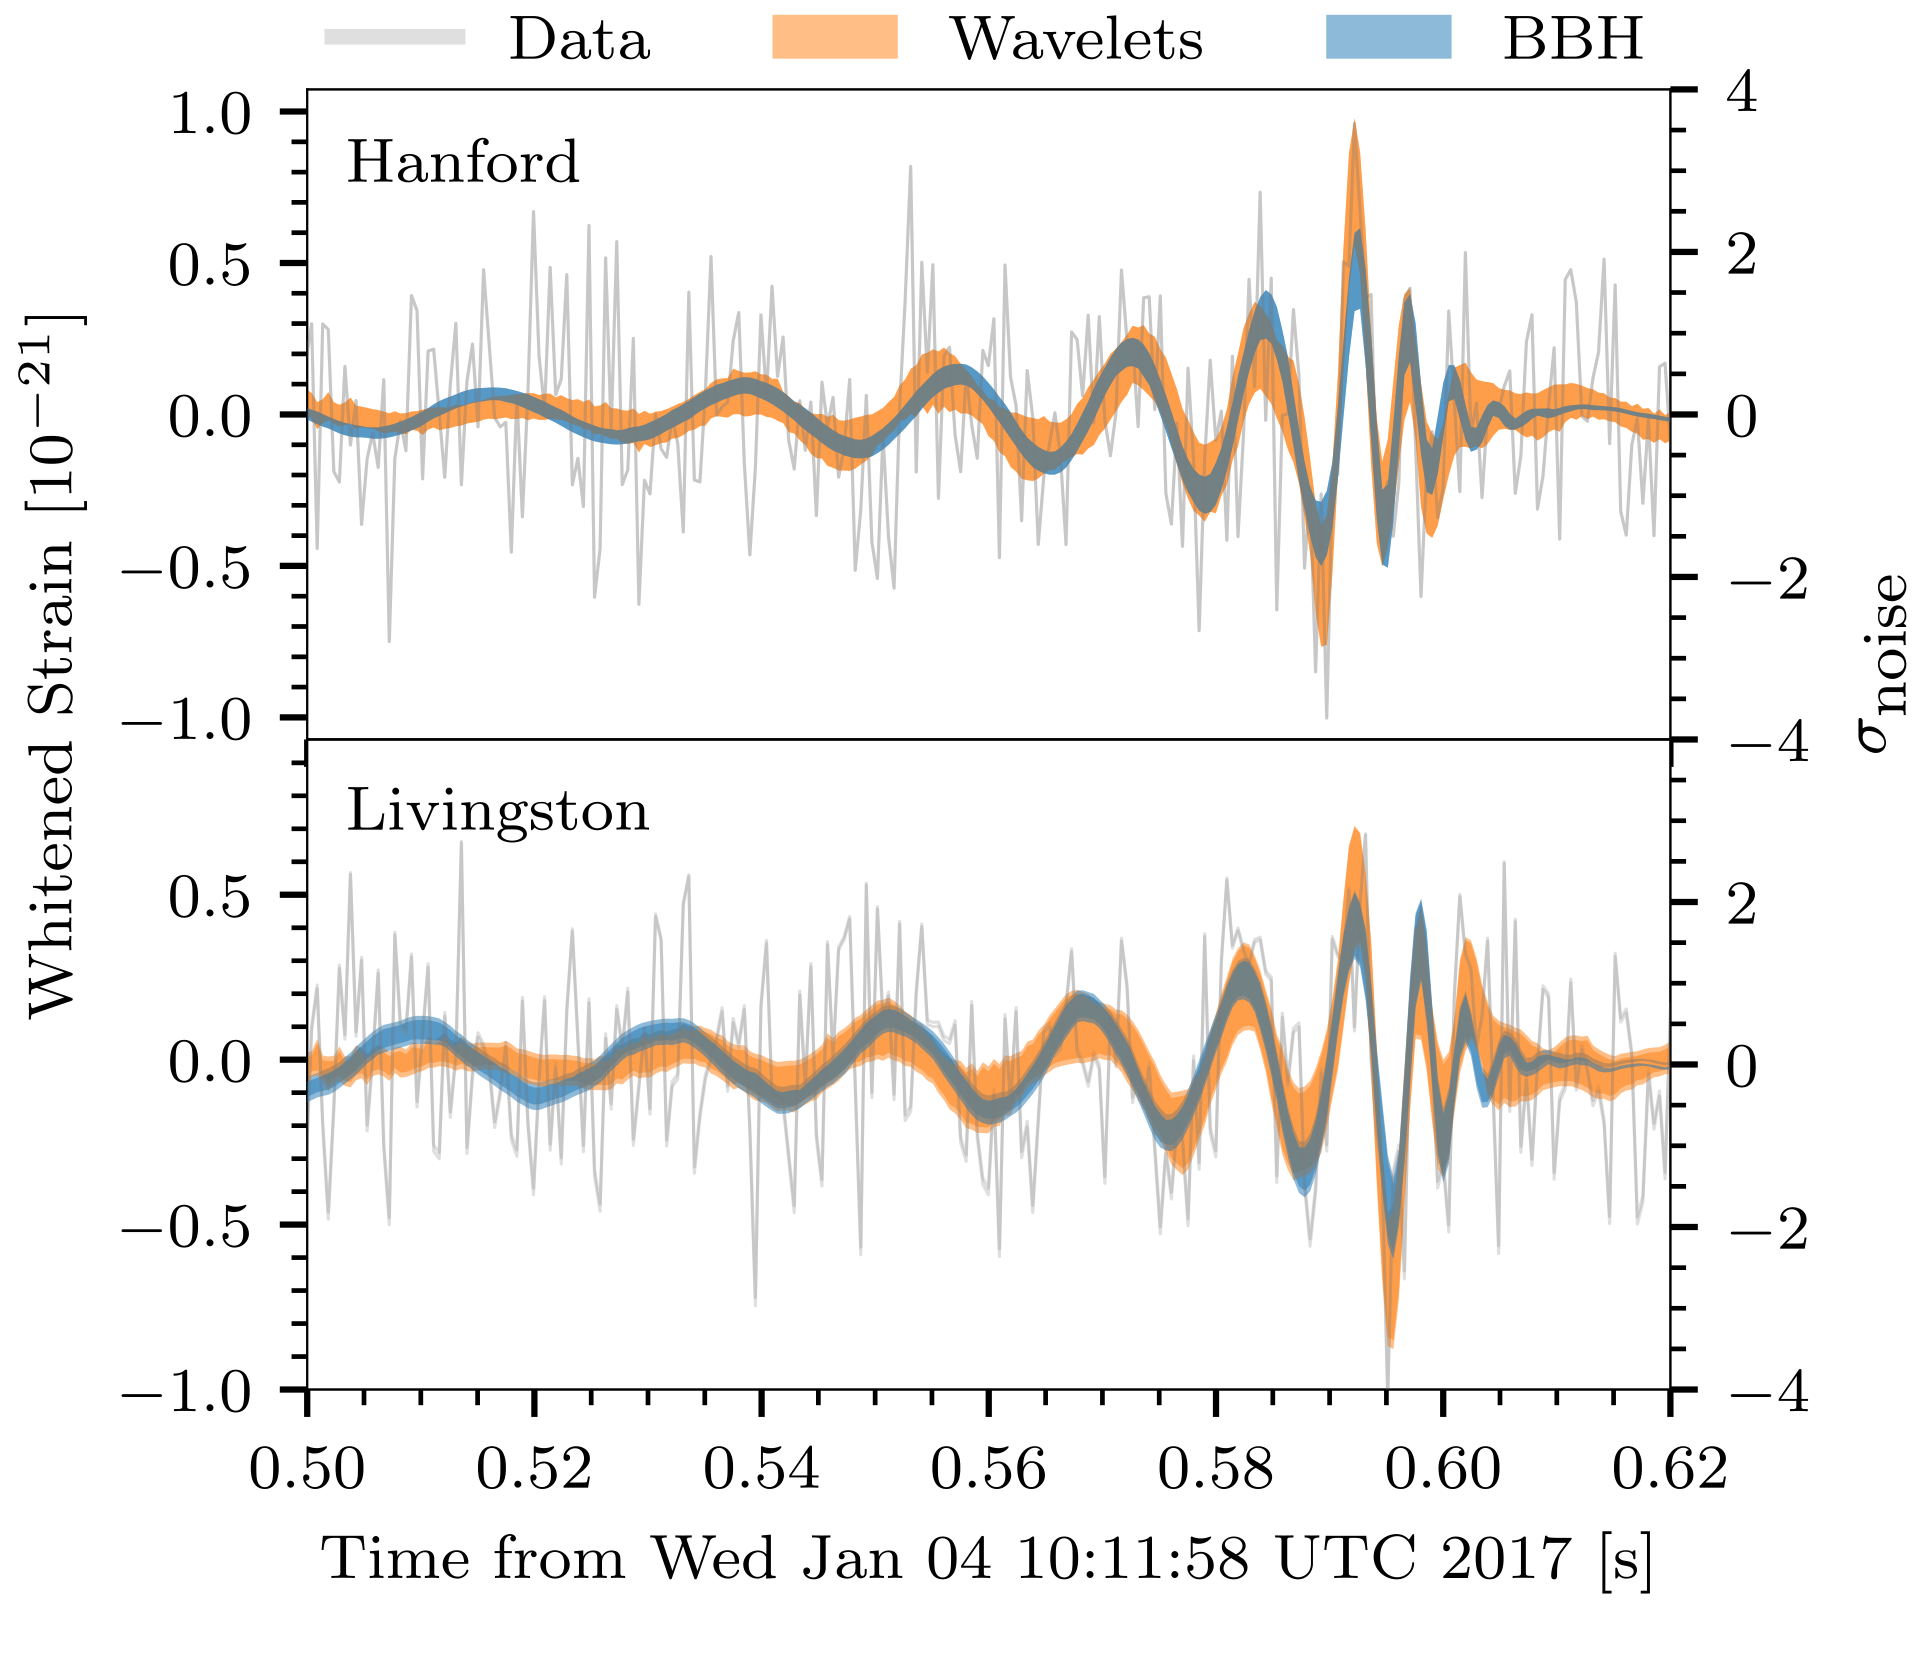
\includegraphics[width=0.45\textwidth]{Figures/GW170104_waveform_reconstructions.svg.png}
	\caption{Treated data and reconstructed signal for GW170104. This figure has been taken from \cite{LIGOScientific:2017bnn}.}
	\label{fig:GW170104Reconstructed}
\end{figure}

\section{Results \& Discussion}
\label{sec:results}
We begin by considering \texttt{tensorflow.keras}'s \texttt{SimpleRNN} on a set of synthetic GW signals for various combinations of the learning rate $\eta$ and $L^2$ regularization parameter $\lambda$ as shown in Fig. \ref{fig:PhiShowcase}. Here we have used 50 epochs for both the figures, where the upper plot uses a dynamical class weights with $\phi=1.4$ and the lower plot uses static class weights, i.e. $\phi=1$. The difference for high $\lambda$ and suboptimal $\eta$ can be seen to be relatively small between the two. In both the cases, large $\lambda$ corresponds to underfitting the model with the high suppression for the weights, and too high (low) value for the initial learning rate causes the model to overshoot (undershoot) the desired minima. For the combinations of $\eta$ and $\lambda$ where the model performs well, we see that there is a clear distinction between the two figures. The model performs much better when it initially starts with higher class weights for the signal class.
\begin{figure}[ht!]
	\begin{subfigure}{0.499\textwidth}
		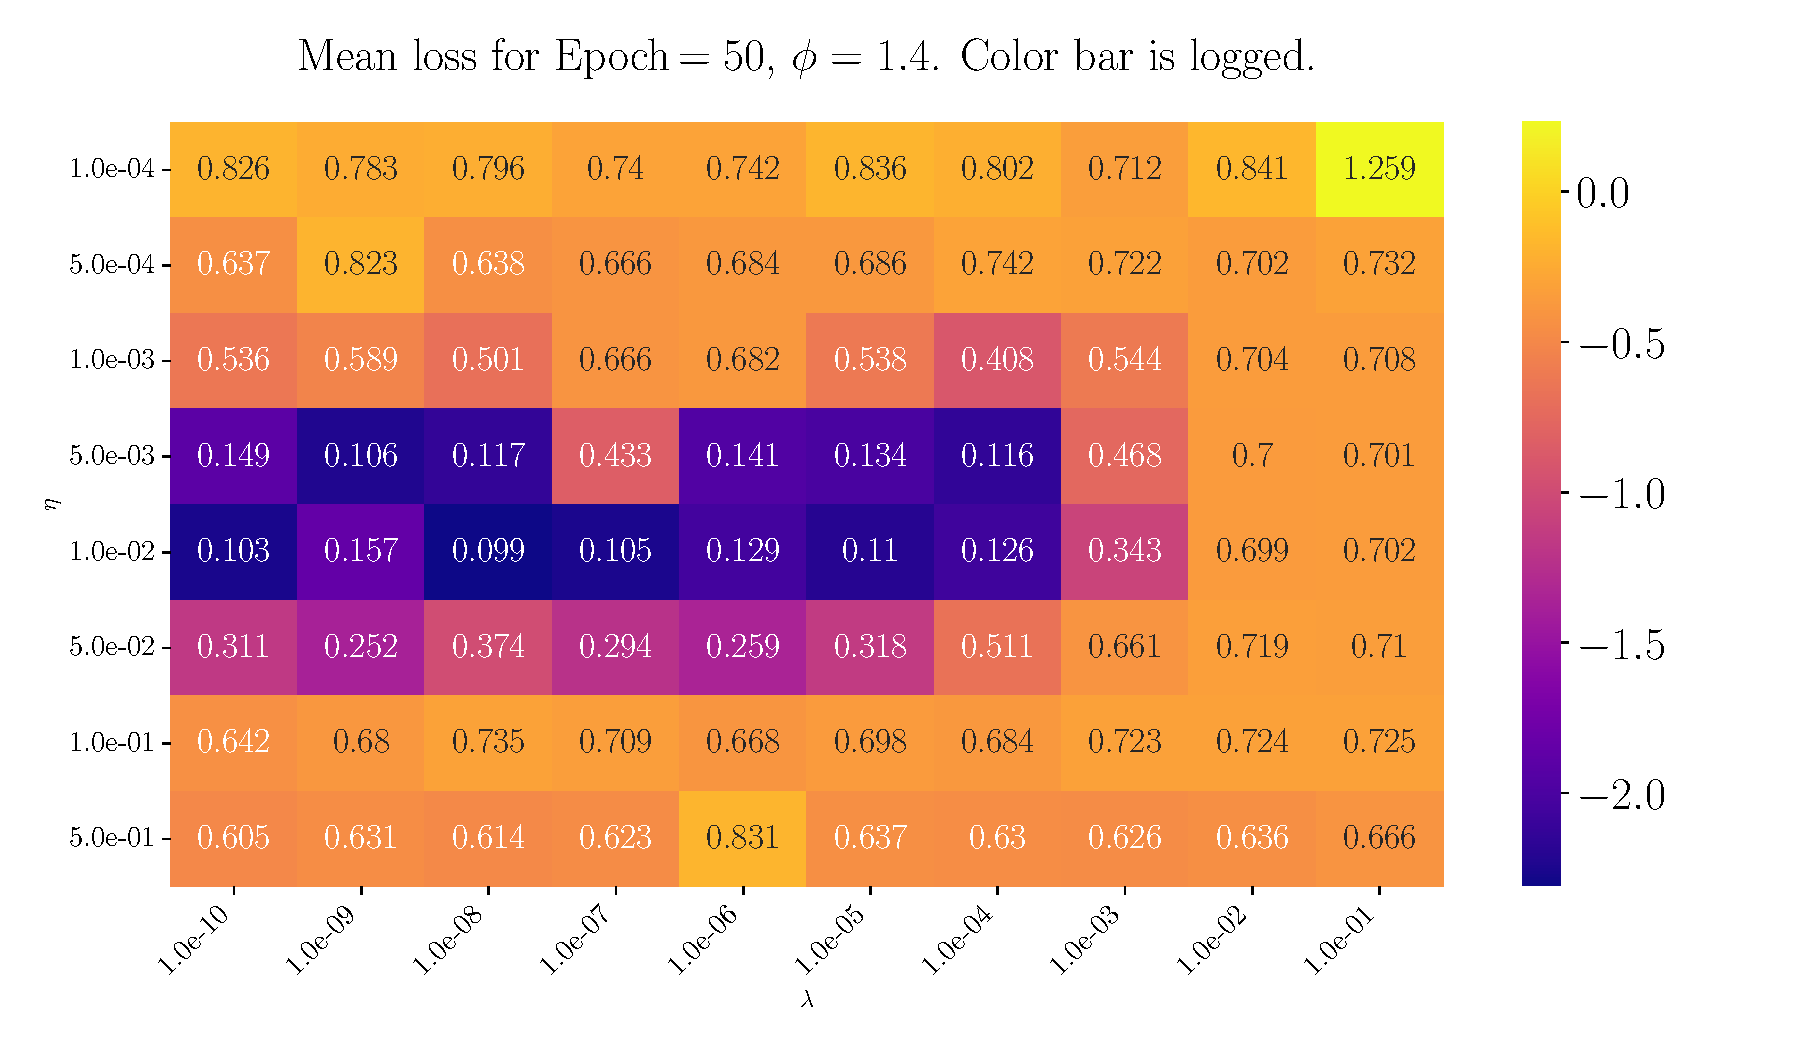
\includegraphics[width=\textwidth]{Figures/2D_Plot_Loss_Epoch50_Boost1.4.pdf}
	\end{subfigure}
	\newline
	\begin{subfigure}{0.499\textwidth}
		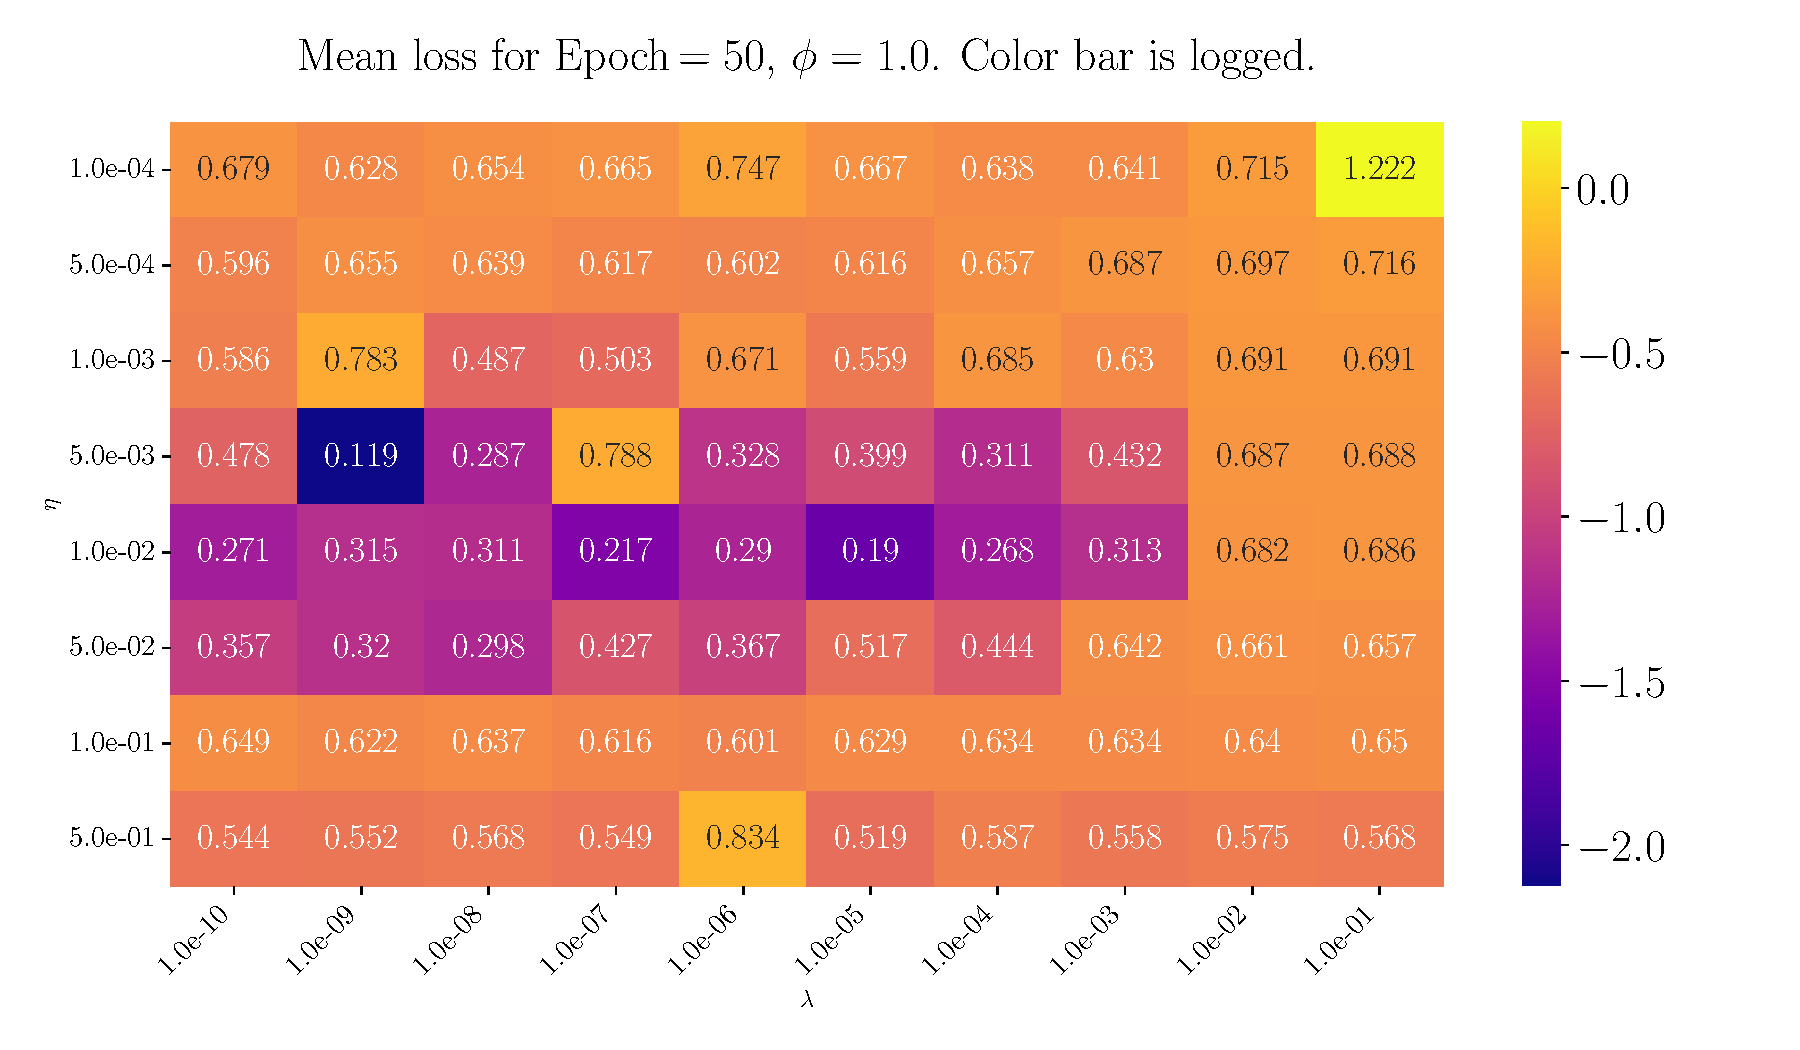
\includegraphics[width=\textwidth]{Figures/2D_Plot_Loss_Epoch50_Boost1.0.pdf}
	\end{subfigure}
	\caption{Average test loss for the $5$-fold cross validation using \texttt{tensorflow.keras}' \texttt{SimpleRNN} for various parameter combinations with 50 epochs. These plots have been chosen to show the effect of an ideal initial boost, $\phi=1.4$, compared to the simpler case $\phi=1$ which corresponds to static, but still balanced, class weights. Note that we have taken the logarithm of the colorbar to get more sensitivity at lower loss.}
	\label{fig:PhiShowcase}	
\end{figure}

The particular example with $\eta=0.01$, $\lambda=10^{-8}$, $\phi=1.4$ with 50 epochs for SNR $\sim100$ is given in Fig.~\ref{fig:bestPred}. Here we have shaded the region in red where the RNN predicted a signal in two neighboring points. The blue line corresponds to the signal itself, whilst the green line is the labels. Here we have much more than just ideal conditions with a rather large SNR, so obviously the task is not nearly as difficult as actual GW events. 
\begin{figure}
	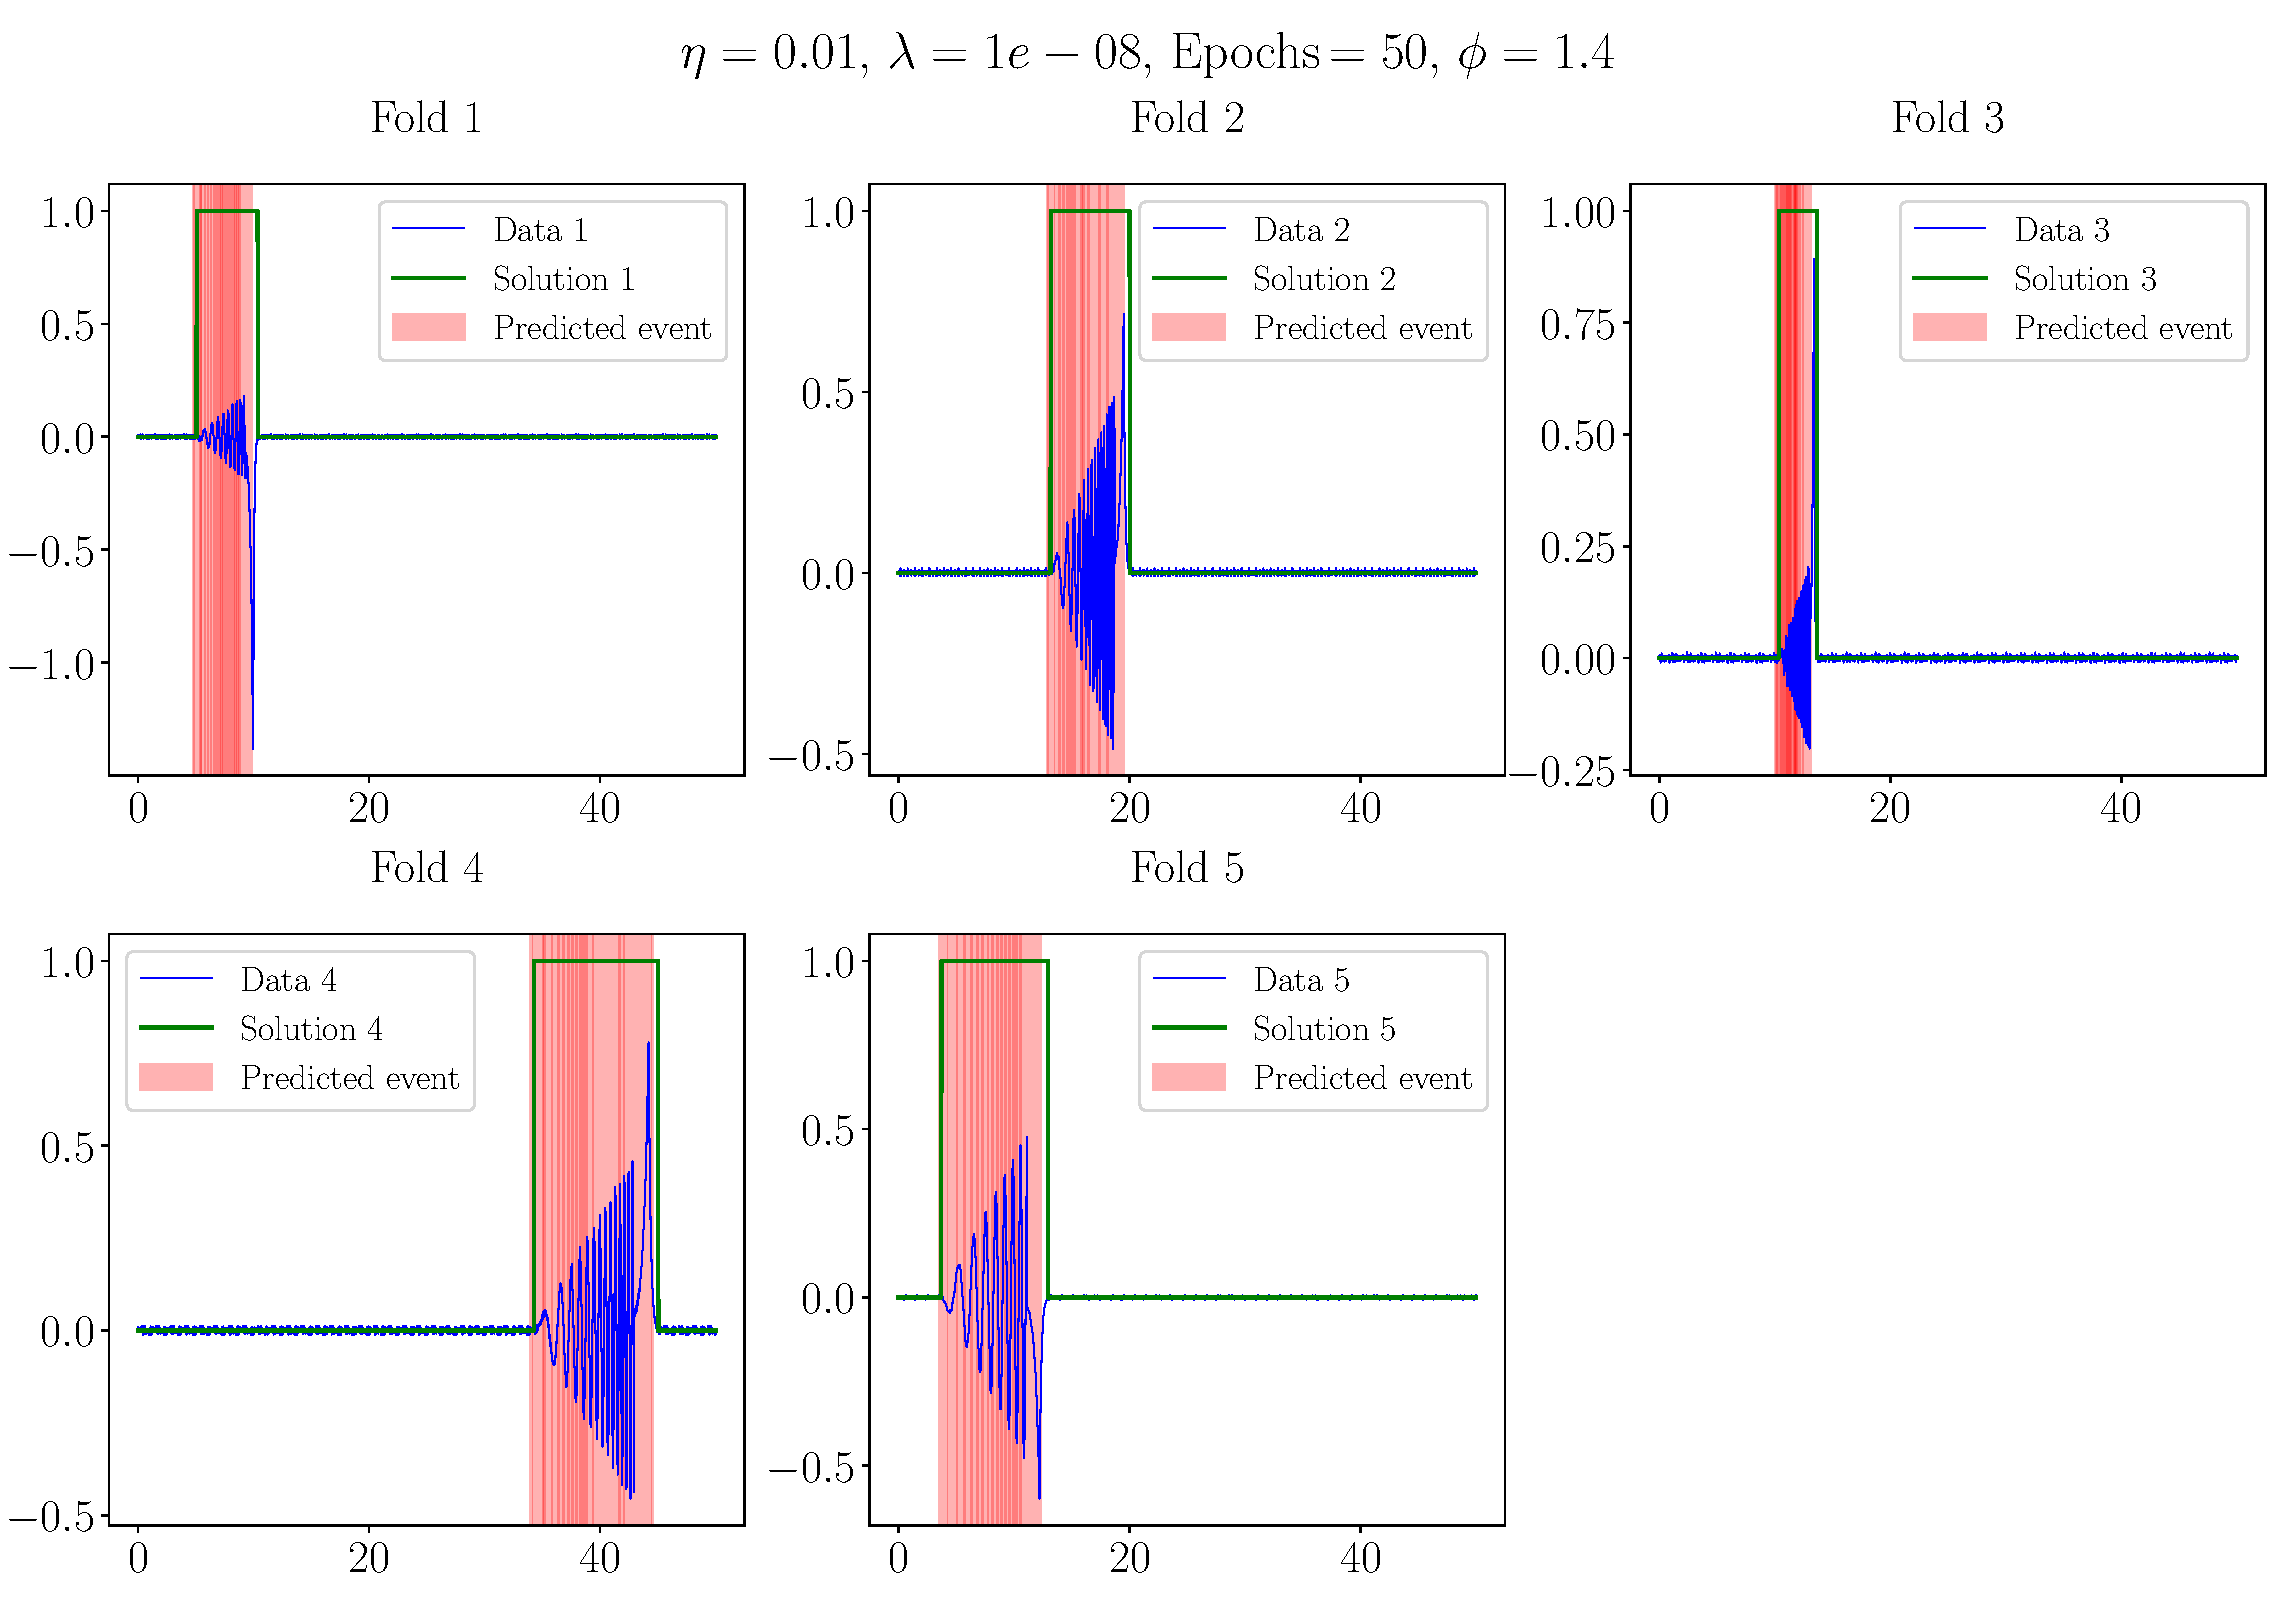
\includegraphics[width=0.49\textwidth]{Figures/BestPrediction_Epochs50_Phi1.4.pdf}
	\caption{Keras RNN with $\eta=0.01$, $\lambda=10^{-8}$, $\phi=1.4$ with 50 epochs for SNR $\sim100$. The blue line corresponds to the generated data, the green line is the labels whilst the shaded red regions are where the RNN predicted a signal. The $x$- and $y$-axes correspond to the time and strain respectively.}
	\label{fig:bestPred}
\end{figure}

We then tried to up the difficulty, lowering the SNR to $\sim15$, which is roughly the range of a treated GW event. This however lead to results so poor that guessing randomly would give a better loss. 

For the CNN however we could lower the SNR to as low values as $X$ whilst still having $\alpha$


\section{Conclusion}
As mentioned prior, actual gravitational wave detection is very difficult, and requires advanced techniques such as matched filtering and adaptive noise subtraction. With our limited time and resources we were not able to properly clean the data to perform such an analysis. Thus we simply opted into creating our own signal in a very ideal situation. 

The RNN's both performed appreciably worse than the CNN, even if we spent much more time making the prior work. Whilst our custom RNN is likely a fault of our own implementation, keras' CNN clearly outperformed its own RNN across all metrics, even achieving similar performance with an SNR which is an order of magnitude lower.

In retrospect, GW detection was not ideal for this project as it was simply too difficult given our limited time and expertise on this topic. Once we saw the lack of performance from the RNN's we should have immediately attempted different methods. Whilst we did this in the end, it was however too late to do a proper analysis to find optimal parameters for the CNN.

% Bibliography
\bibliographystyle{JHEP}
\bibliography{project3}
	
\end{document}